\documentclass{standalone}

\usepackage{pgfplots,mathtools}
\pgfplotsset{compat=newest}

\usetikzlibrary{intersections}

\let\Re\relax
\DeclareMathOperator{\Re}{Re}

\begin{document}
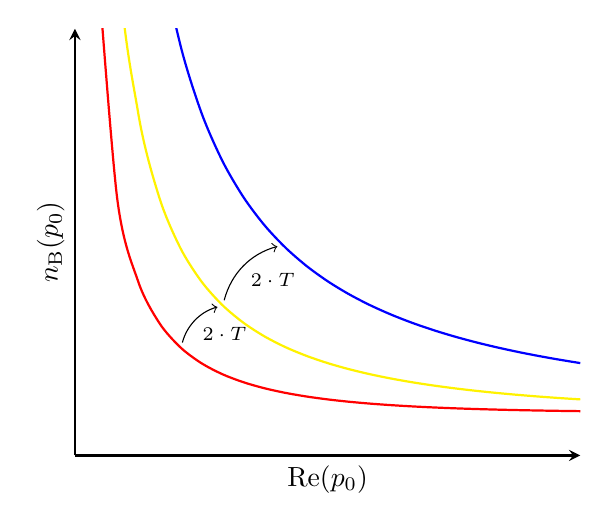
\begin{tikzpicture}
  \begin{axis}[
      domain = 0:2,ymax = 5,
      xlabel = $\Re(p_0)$,
      ylabel = $n_\text{B}(p_0)$,
      ticks=none,smooth,
      thick,axis lines = left,
      every tick/.style = {thick},
      width=8cm,height=7cm]

    \def\nB#1{1/(e^(x/#1) - 1) + 1/2}

    \addplot[name path=T1,color=red]{\nB{0.5}};

    \addplot[name path=T2,color=yellow]{\nB{1}};

    \addplot[name path=T3,color=blue]{\nB{2}};

    \addplot [draw=none,name path=aux] {3*x};

  \end{axis}

  \draw[shorten >=2,shorten <=2,name intersections={of=T1 and aux,name=int1},name intersections={of=T2 and aux,name=int2}] (int1-1) edge[->,bend left] node[midway,below right=-1pt,font=\scriptsize] {$2 \cdot T$} (int2-1);

  \draw[shorten >=2,shorten <=2,name intersections={of=T3 and aux,name=int3}] (int2-1) edge[->,bend left] node[midway,below right=-1pt,font=\scriptsize] {$2 \cdot T$} (int3-1);

\end{tikzpicture}
\end{document}
